%\cleardoublepage
%\phantomsection
\chapter{Hybrydowa metoda śledzenia ruchu człowieka}\label{chap:hybrid}

Prezentowana w niniejszej dysertacji hybrydowa metoda śledzenia ruchu człowieka, wykorzystuje dwa rodzaje urządzeń pomiarowych: kontroler Microsoft Kinect oraz czujniki inercyjne - akcelerometr i żyroskop, które zostały scharakteryzowane w rozdziale \ref{chap:characteristics}. Mając na uwadze dokładność danych przesyłanych przez każde z zastosowanych urządzeń pomiarowych oraz ograniczenia w ich działaniu, takie jak wrażliwość na występowanie okluzji sensora głębi, czy ograniczona liczba stopni swobody układów inercyjnych, opracowana przeze mnie hybrydowa metoda śledzenia ruchu człowieka umożliwia ograniczenie wpływu niedoskonałości każdego ze stosowanych urządzeń. Autorskie połączenie danych (ang. \textsl{data fusion}) z kontrolera Kinect i czujników inercyjnych poprawia precyzję szacowania położenia stawów, a co za tym idzie wpływa korzystnie na precyzję śledzenia wykonywanego przez użytkownika ruchu. Ograniczenie wpływu niedoskonałości każdego z wykorzystanych urządzeń pomiarowych na dokładność śledzenia ruchu możliwe jest dzięki temu, że są one względem siebie w pewnym stopniu komplementarne to znaczy, że niedoskonałości występujące w jednym urządzeniu i wpływające np. na brak śledzenia ruchu w jednej z płaszczyzn mogą zostać ograniczone przez wykorzystanie możliwości śledzenia ruchu w tej płaszczyźnie przez drugie z urządzeń.\\
Proces łączenia danych uzyskanych z kontrolera Kinect i z czujników inercyjnych podzielony został na kilka etapów, z których część jest \emph{przeprowadzona jednokrotnie} na samym początku, a część jest powtarzana w trakcie śledzenia ruchu. Kolejno wykonywanymi etapami są:
%kolor nie jest tutaj najlepszym znacznikiem, bo ktoś to może wydrukować w skali szarości i nic nie zrozumie. Może podejśc do tego trochę algorytmicznie/blokowo to jest bardziej inżynierskie podejście wtedy od razu można podac podrozdziały, w których są opisane poszczególne etapy.
\begin{enumerate}
	\item \emph{\textcolor{blue}{Inicjalizacja czujników inercyjnych,}}
	\item \emph{\textcolor{blue}{Inicjalizacja filtrów łączących dane z akcelerometru i żyroskopu,}}
	\item Odszumienie danych z czujników inercyjnych oraz z kontrolera Kinect,
	\item \emph{\textcolor{blue}{Synchronizacja czasowa sygnałów z czujników inercyjnych oraz z kontrolera Kinect,}}
	\item Łączenie danych z czujników inercyjnych oraz z kontrolera Kinect,
	\item Oszacowanie położenia stawów.
\end{enumerate}

Powyższe kroki omówione zostały w dalszej części rozdziału.\\

Zadaniem omawianej w niniejszym rozdziale hybrydowej metody śledzenia ruchu człowieka jest oszacowanie w chwili czasu $t$ położenia wybranych stawów szkieletu postaci w (przestrzeni trójwymiarowej opisanej układem współrzędnych $X\quad Y\quad Z$)

(zamiast tego co w nawiasie musisz wpisać globalny układ współrzędnych lub układ współrzędnych kontrolera Kinect lub też odwołać się do jakiegoś układu, który jest na rysunku wcześniej, np. przy opisie postaci) ($P^F_t = \begin{bmatrix}p^F_x\\p^F_y\\p^F_z\end{bmatrix}_t$) (skąd symbol F? poza tym takie pionowe macierze niedobrze wyglądają w tekście. Trzeba to zebrać jako równania poza tekstem i się do nich odwołać w tekście pracy, np. eg. ??). 

W zakresie czujnika inercyjnego szacowanie położenia stawu odbywa się na podstawie pomiaru sił działających na akcelerometr w każdej z trzech osi 
(eq. ?? zamiast takiej macierzy, czyba że będzie pozioma) 
($A = \begin{bmatrix}a_x\\a_y\\a_z\end{bmatrix}$), pomiaru prędkości kątowych z jakimi porusza się żyroskop względem każdej z osi (którego układu współrzędnych?) ($G = \begin{bmatrix}g_x\\g_y\\g_z\end{bmatrix}$) oraz aktualnej temperatury pracy czujników inercyjnych ($T$). W przypadku kontrolera Kinect pobierane są pozycje dwóch stawów (dlaczego przy ogólnym rozważaniu tylko dwóch?), stawu którego pozycja będzie szacowana ($P^K_{i+1} = \begin{bmatrix}p^{K_{i+1}}_x\\p^{K_{i+1}}_y\\p^{K_{i+1}}_z\end{bmatrix}$) oraz stawu będącego jego rodzicem w modelu szkieletowym Kinecta (rys. \ref{fig:characteristics:kinect:skeleton}, $P^K_0 = \begin{bmatrix}p^{K_i}_x\\p^{K_i}_y\\p^{K_i}_z\end{bmatrix}$) (szkoda, że na rysunku do którego się odwołujesz sa inne oznaczenia niż używasz w tekście i we wzorze). Oszacowanie pozycji stawu $P^F_t$ odbywa się z pewnym interwałem czasowym $\Delta t$ określającym czas pomiędzy kolejnymi aktualizacjami pomiarów kontrolera Kinect (a co z interwałem czasowym urządzenia inercyjnego). Biorąc pod uwagę powyższe, oszacowanie pozycji wybranego stawu przez omawianą hybrydową metodę śledzenia ruchu człowieka można wyrazić za pomocą wzoru \eqref{eq:methodFormula}.
%mam zastzrzeżenie, czy ten wzór powinien mieć tylko dwa stawy czy może więcej oraz czy częstotliwość pomiaru kinecta jest właściwym argumentem bo przecież dla poojedynczego pomiaru pozycji stawu nie jest istotny interwał pracy Kinecta, czy może kwestie opóźnień przesyłu danych pomiędzy urządzeniami czy inne aspekty synchronizacji/opóxnień  
\begin{equation}
	f(A,G,T,P_0^K,P_1^K,\Delta t) => [p_x^F,p_y^F,p_z^F]_t
	\label{eq:methodFormula}
\end{equation}

Wzór \eqref{eq:methodFormula} odnosi się do każdego markera zbudowanego z pary czujników: akcelerometru i żyroskopu (markery inercyjne) umieszczonego na ciele pomiędzy dwoma kolejnymi stawami, których pozycje oszacowane przez kontroler Kinect są argumentami metody. 
%po tym zdaniu śmiem przypuszczać, że podstawowym Twoim problemem jest śledzenie stawu dziecka względem stawu rodzica a nie pozycji stawu w zewnętrznym układzie wspólrzednych. Trzeba to wyjaśnić 

Eksperymenty badawcze przeprowadzone w niniejszej pracy śledziły (sam eksperyment nic nie śledzi) ruch ręki z wykorzystaniem dwóch markerów inercyjnych, jednego umieszczonego na ramieniu (pomiędzy stawem barkowym a stawem łokciowym) oraz drugiego umieszczonego na przedramieniu, pomiędzy stawem łokciowym a stawem nadgarstkowym. Schemat umieszczenia markerów inercyjnych przedstawia rysunek \ref{fig:hybrid:imuMarkerPlacementSample}.
%opis eksperymentów powinien być w częsci testowej a nie w opisie metody
\begin{figure}[!htp]
	\centering	
	\includegraphics[width=0.75\textwidth]{images/imuArm.png}
	\caption{Schemat umieszczenia markerów inercyjnych na potrzeby eksperymentów badawczych opisanych w niniejszej pracy.}
	\label{fig:hybrid:imuMarkerPlacementSample}
\end{figure}
%identyczny ryzunek był w drugim rozdziale. Po co to powtarzać. Poza tym to część

\section{Format danych używany przez urządzenia pomiarowe}
\subsection{Kontroler Kinect}
Kontroler Kinect w ramach pakietu pomiarów, rejestrowanego z częstotliwością $30 Hz$, udostępnia 3 kategorie danych dotyczących obserwowanej sceny: obraz z kamery RGB, mapę głębi sceny oraz model szkieletowy postaci widocznej na scenie. Kontroler Kinect może jednocześnie zrekonstruować modele szkieletowe dwóch postaci i śledzić ich kolejne pozy, rejestrując tym samym ich ruch. W zależności od potrzeb, aplikacja wykorzystująca kontroler Kinect może uzyskać wszystkie 3 kategorie danych jednocześnie lub wybrać tylko te z nich, które potrzebuje do swojego działania. Opisywana w niniejszej dysertacji hybrydowa metoda śledzenia ruchu kończyn człowieka bazuje na informacji dotyczącej modelu szkieletowego śledzonej postaci wybierając z pełnego modelu tylko informacje związane z wybranymi stawami reprezentującymi śledzoną kończynę. (niezbędnymi do prawidłowego działania opisywanej metody - niezbędne jest to co jest śledzone, ale samam metoda nie ma ograniczeń w tym względzie). Przykładowo w przypadku śledzenia ruchu prawej ręki są to oba stawy barkowe, prawy staw łokciowy oraz prawy staw nadgarstkowy. Każdy staw reprezentowany jest przez 3 współrzędne określające jego położenie w przestrzeni (istotne jest podanie w jakim układzie wspólrzędnych?!) oraz informacje o stanie śledzenia tego stawu (podać jakie moga być stany!). Na podstawie współrzędnych stawów barkowych postaci obliczany jest kąt obrotu sylwetki względem Kinecta (wzór \eqref{eq:characteristics:kinect:bodyRotationAngle}. Dodatkowo każdy pakiet danych zawiera informacje o swoim numerze, znacznik czasu wygenerowany przez kontroler Kinect oraz godzinę odebrania danych na komputerze, do którego podłączone jest to urządzenie.

\subsection{Czujniki inercyjne}
Moduł inercyjny zbudowany został z czujników inercyjnych: akcelerometru i żyroskopu, podłączonych bezpośrednio do jednostki centralnej opartej na platformie Arduino (rys. ??). Zadaniem jednostki centralnej jest odczyt danych z czujników, sformatowanie ich i wysłanie z wykorzystaniem technologii Bluetooth do komputera PC, gdzie następuje dalsze ich przetwarzanie. Odczyt pakietu danych z pojedynczego modułu obejmuje zestaw pomiarów udostępnionych przez żyroskop (3 wartości obrotu, po jednej dla każdej z osi), zastaw pomiarów z akcelerometru (3 wartości przyspieszenia) oraz pomiaru temperatury czujników. Wszystkie pomiary przesyłane są jako 16-bitowe liczby całkowite ze znakiem i pomiary ze wszystkich podłączonych modułów wysyłane są do komputera PC jednocześnie. Przesyłane wartości muszą być następnie skonwertowane do jednostek odpowiadających wielkościom fizycznym mierzonym przez poszczególne czujniki tj. dla żyroskopu są to stopnie na sekundę ($\degree/_s$), dla akcelerometru -- jednostki grawitacji ($g$)(jednostką przyspieszenia ziemskiego sa metry na sekunde kwadrat - dlaczego nie jest podane jawnie?)  a dla temperatury stopnie Celsjusza ($\degree C$). W przypadku danych z czujników inercyjnych konwersja polega na podzieleniu wartości bezpośredniego odczytu z czujników przez współczynniki odpowiednie dla zakresu pracy tych czujników. Tabele \ref{tab:hybrid:gyroRangeFactors} oraz \ref{tab:hybrid:accRangeFactors} przedstawiają zestawienie współczynników wykorzystywanych do konwersji pomiarów z czujników inercyjnych (one powinny mieć symbole skoro później te symbole sa używane we wzorach). Jak już zostało to zaznaczone wcześniej, w trakcie prowadzonych eksperymentów badawczych, zakres pracy akcelerometru został ustalony na $\pm4g$ natomiast żyroskopu na $\pm500\degree/_s$. Zakresy dla czujników modułów inercyjnych zostały dobrane (przyjęto podobne wartości) na podstawie parametrów czujników inercyjnych zastosowanych w kontrolerze ruchu Nintendo Wii Remote Plus.

\begin{table}[!htp]
	\centering
	\caption{Współczynniki przeliczenia bezpośrednich pomiarów żyroskopu w zależności od zakresu pracy}	
	\label{tab:hybrid:gyroRangeFactors}	
	\begin{tabular}{|l|c|}
		\hline
		Zakres pomiaru                     & Współczynnik  \\ \hline
		$\pm250\frac{\degree}{s}$          & $131.0$         \\ \hline
		\textbf{$\pm500\frac{\degree}{s}$} & \textbf{$65.5$} \\ \hline
		$\pm1000\frac{\degree}{s}$         & $32.8$          \\ \hline
		$\pm2000\frac{\degree}{s}$         & $16.4$          \\ \hline
	\end{tabular}
\end{table} 		
\begin{table}[!htp]
	\centering
	\caption{Współczynniki przeliczenia bezpośrednich pomiarów akcelerometru w zależności od zakresu pracy}
	\label{tab:hybrid:accRangeFactors} 
	\begin{tabular}{|l|c|}
		\hline
		Zakres pomiaru   & Współczynnik  \\ \hline
		$\pm2g$          & $16384$         \\ \hline
		\textbf{$\pm4g$} & \textbf{$8192$} \\ \hline
		$\pm8g$          & $4096$          \\ \hline
		$\pm16g$         & $2048$          \\ \hline
	\end{tabular}
\end{table} 

Konwersja pomiaru temperatury czujników ($T_{raw}$) do wartości wyrażonej w $\degree C$ ($T_{deg}$) wymaga zastosowania wzoru \eqref{eq:hybrid:tempEquation} wynikającego ze specyfikacji zastosowanego układu elektronicznego IvenSense MPU-6050. Wartości stałe zastosowane w tym wzorze związane są z rozdzielczością pomiarów wykorzystanego w tym układzie elektronicznym termometru (wartość = 340.0) oraz ze stałego przesunięcia dla temperatury $0 \degree C$ (wartość = 36.53)

\begin{equation}
	T_{deg} = 36.53 + T_{raw} / 340.0
	\label{eq:hybrid:tempEquation}
\end{equation}

Do danych pobranych ze wszystkich podłączonych modułów inercyjnych, podobnie jak w przypadku danych z Kinecta, dołączone są znaczniki czasowe zarówno ustawiane przez urządzenie, jak i przez komputer PC w momencie odbioru danych oraz numeracja kolejnych pakietów danych.

\section{Kalibracja}
W proponowanym systemie czujniki inercyjne wymagają kalibracji przy każdym uruchomieniu. Kalibracja Kinecta nie jest wymagana, a jedyne co należy zrobić to upewnić się, że kąt nachylenia kamery pozwala na obserwację śledzonej postaci.

Kalibracja czujników inercyjnych przebiega dwuetapowo w następującej kolejności:
\begin{enumerate}
	\item {Wyznaczenie współczynników korekty pomiarów czujników inercyjnych dla wartości spoczynkowych} (rozumiem, że korekcie podleagą te współczynniki, które są w dwóóch powyższych tabelach, czy innych?)
	\item {Inicjalizacja filtru Madgwicka wyznaczającego orientację sensora na podstawie danych z czujników inercyjnych}
\end{enumerate}

Krok pierwszy służy do wyznaczenia wartości korekty pomiarów dla urządzenia w spoczynku. W trakcie tego kroku kalibrowane czujniki należy umieścić możliwie jak najbardziej poziomo tak, żeby oś $Z$ sensora była równoległa do kierunku działania siły grawitacji. Wówczas wartości rzeczywiste jakie powinny wskazywać czujniki dla każdej z osi $(X\quad Y\quad Z)$ wynoszą odpowiednio $(0g\quad 0g\quad 1g)$ dla akcelerometru oraz $(0\degree/_s\quad 0\degree/_s\quad 0\degree/_s)$ dla żyroskopu. W praktyce jednak, ze względu na zaszumienie danych i brak możliwości całkowitego ich oczyszczenia, wartości idealne nie są osiągalne. W związku z tym, algorytm odpowiedzialny za kalibrację (jaki to algorytm? Czy można go podać?) działa iteracyjnie (indeks iteracji = $j$) tak długo, aż osiągnie średni błąd pomiaru ($\overline{v}$) (wprowadzone jest v bez powiązania z danymi z czujników!) nie większy niż akceptowalna wartość graniczna błędu ($v_{th}$) (skąd się wzięła wielkość v skoro wczesniej nie była podana). Efektem działania algorytmu kalibracji (jaki to algorytm?) jest wartość współczynnika korekty pomiaru ($s_{off}$) (jak sie ma wczesniejszy wspólczynnik korekty do współczynników kalibracji?) pozwalająca osiągnąć założoną dokładność pomiarów. 
Kolejność wykonywanych obliczeń w omawianym algorytmie kalibracji jest następująca: najpierw obliczana jest średnia wartość błędu pomiarów ($v$) przy aktualnej wartości współczynnika korekty, a następnie, jeśli to konieczne, aktualizowany jest wspomniany współczynnik (symbole, bo nie wiadomo o których wspólczynnikach piszesz). W przypadku pierwszej iteracji ($j = 0$) (czy nie można iteracji od 1?) wartość współczynnika korekty pomiarów wynosi 0 zaś średni błąd pomiarów czujnika inercyjnego wyrażony jest wzorami \eqref{eq:hybrid:IMUCalibration:1} i \eqref{eq:hybrid:IMUCalibration:2} (ten wzór nie jest dla j=0, czyli nieprawda). Jeśli uzyskana średnia wartość błędów pomiaru przekracza dopuszczalną wartość (gdzie jest równanie?) aktualizowany jest współczynnik korekty (który?). Wyznaczenie współczynnika korekty wykorzystuje różnicę jaka jest pomiędzy teoretyczną, idealną wartością jaką powinien w danym położeniu wskazywać czujnik ($\nu$) (symbol łatwo pomylić z $v$!) a uzyskiwanym średnim błędem pomiarów kalibrowanego czujnika. Aktualizacja współczynników korekty wyrażona jest wzorami \eqref{eq:hybrid:IMUCalibration:3} i \eqref{eq:hybrid:IMUCalibration:4}.

\begin{subnumcases}{\overline{v}_j =}
	\frac{1}{n}\sum_{i=1}^{n}{v}                       & $j = 0$ \label{eq:hybrid:IMUCalibration:1}\\
	\frac{1}{n}\sum_{i=1}^{n}{v - {s_{off}}_{j-1}}            & $j > 0$ \label{eq:hybrid:IMUCalibration:2}
\end{subnumcases}
\begin{subnumcases}{{s_{off}}_j =}                                        
	\frac{\nu - \overline{v}_0}{8}                        & $j = 0$ \label{eq:hybrid:IMUCalibration:3}\\
	{s_{off}}_{j-1} - \frac{\nu - \overline{v}_j}{v_{th}} & $j > 0$ \label{eq:hybrid:IMUCalibration:4}
\end{subnumcases}



Algorytm kalibracji czujników stosowany jest osobno do każdej osi każdego z czujników co dla jednego modułu inercyjnego złożonego z akcelerometru i żyroskopu daje konieczność przeprowadzenia kalibracji 6 pomiarów (może 6 mierzonych parametrów? Swoją drogą dlaczego nie 7?). Aby uznać dany moduł za skalibrowany wszystkie 6 pomiarów (6 mierzonych parametrów) musi jednocześnie osiągnąć średnią wartość błędu poniżej zakładanych dla tych pomiarów maksymalnych wartości błędu ($v_{th}$). Kalibracja modułu zajmuje zwykle około 10 iteracji, natomiast zdarzały się sytuacje, w których trwało to ponad 2 razy dłużej. Było to zazwyczaj spowodowane poruszeniem modułu w trakcie kalibracji.

Kolejnym krokiem jest inicjalizacja filtru Madgwicka łączącego dane z czujników inercyjnych w celu wyznaczenia ich orientacji w przestrzeni. Łączenie to ma na celu ograniczenie dryfu żyroskopu za pomocą pomiarów akcelerometru, a następnie wyznaczenie orientacji przestrzennej modułu inercyjnego. W literaturze najczęściej spotykanym filtrem wykorzystywanym do tego celu jest filtr Kalmana \cite{Sasiadek2000, Sabatini2011, Mau2005, Qingming2014} (opis filtrów Kalmana można znaleźć w dodatku \ref{chap:appx:filters}). W roku 2010 Sebastian Madgwick opublikował raport ze swoich badań, w którym przedstawił wzór autorskiego filtra łączącego dane z akcelerometru i żyroskopu oraz wariant uzupełniony o dane z magnetometru,  przedstawiający orientację urządzenia pomiarowego zbudowanego z tych czujników w postaci kwaternionów \cite{Madgwick2010, Madgwick2011}. W przytoczonych pracach opublikowane zostały także wyniki testów porównujących zaproponowany filtr z filtrem Kalmana, z których wynika, że filtr Madgwicka osiąga lepsze wyniki niż filtr Kalmana w wyznaczaniu orientacji przestrzennej na podstawie pomiarów z akcelerometru, żyroskopu i opcjonalnie z magnetometru. W opisywanej w tym rozdziale autorskiej hybrydowej metodzie śledzenia ruchu kończyn (dodałem kończyn, bo to chyba jest precyzyjniej) człowieka, wykorzystany został filtr Madgwicka ($m(\ldots)$) opisany wzorem \eqref{eq:hybrid:magwickFormula}. 

\begin{equation}
	Q_t = m(Q_{t-1}, A, G, dt, \beta) 
	\label{eq:hybrid:magwickFormula}
\end{equation}
gdzie
\begin{conditions}
	Q & kwaternion reprezentujący orientację czujnika w przestrzeni wyrażony jako $\left[q_w\quad q_x\quad q_y\quad q_z\right]$\\
	A & wektor reprezentujący pomiar akcelerometru $\left[a_x\quad a_y\quad a_z\right]$\\
	G & wektor reprezentujący pomiar żyroskopu $\left[g_x\quad g_y\quad g_z\right]$\\
	dt & czas pomiędzy kolejnymi pomiarami wyrażony w sekundach\\
	\beta & współczynnik filtracji\\
\end{conditions}
%upewnij się, że powyższe oznaczenia dla czujników sa spójne z wczesniejszymi oznaczeniami
Inicjalizacja filtru Madgwicka odbywa się poprzez jego wielokrotne zastosowanie dla uśrednionych pomiarów z czujników inercyjnych znajdujących się i dokonujących pomiary w stanie spoczynku. W trakcie inicjalizacji filtru Madgwicka powinien być on zastosowany taką liczbę razy jakiej liczności była próbka do wyznaczenia uśrednionych wartości pomiarów czujników tj. jeśli średnie wartości pomiarów były wyznaczone z próbki zawierającej 1000 wartości to w ramach inicjalizacji filtr Madgwicka powinien być zastosowany 1000-krotnie dla uśrednionych danych.\\

Zgodnie z zaleceniami twórcy tej metody, w trakcie inicjalizacji, wartość współczynnika filtracji $\beta$ powinna być relatywnie wysoka. W opisywanej metodzie, w trakcie tego procesu $\beta = 2$. Po zakończeniu inicjalizacji współczynnik $\beta$ zostaje wyznaczony wg wzoru \eqref{eq:hybrid:magwickBetaFormula}. Jest on zależny od średniej wartości szumu błądzenia $\widetilde{\omega}$ (ARW) wyznaczonego dla żyroskopu na podstawie wariancji Allana (dodatek \ref{chap:appx:allan}). W przypadku wykorzystanych czujników wartość ARW wynosi $\widetilde{\omega} = 0.009$, więc współczynnik $\beta = 0.082$

\begin{equation}
	\beta = \sqrt{\frac{3}{4}\widetilde{\omega}}
	\label{eq:hybrid:magwickBetaFormula}
\end{equation}

\section{Korekta danych z urządzeń pomiarowych}

Dane pobrane z czujników inercyjnych oraz z kontrolera Kinect muszą zostać poddane filtracji aby ograniczyć wpływ szumów na uzyskane pomiary. W przypadku czujników inercyjnych, wpływ szumów wynikający z błądzenia losowego zostaje skutecznie ograniczony w trakcie łączenia danych pobranych z akcelerometru z danymi pobranymi z żyroskopu za pomocą filtru Madgwicka, którego wynikiem jest oszacowana orientacja, w jakiej znajduje się dany moduł inercyjny. Ograniczenie wpływu szumów obecnych w danych pomiarowych ma bezpośrednie przełożenie na stabilność i dokładność oszacowanej orientacji. Dla osi $X$ i $Y$, oszacowana wartość orientacji jest stabilna w czasie, a dokładność w stosunku do prawdziwej orientacji markera inercyjnego wyniosła $\pm 2\degree$ (skąd to wiemy?). Oszacowanie orientacji w osi $Z$ odbywa się jedynie na podstawie danych pomiarowych żyroskopu, co powoduje, że uzyskiwany wynik nie jest stabilny w czasie. Analizując wykres (gdzie ten wykres?) przedstawiający wartość oszacowania orientacji w osi $Z$ w czasie dla markera inercyjnego będącego w spoczynku, można zaobserwować ciągłą zmianę wartości tak jakby urządzenie pomiarowe wciąż się obracało. W związku z tym oszacowanie obrotu wokół tej osi jest całkowicie niewiarygodne i nie nadaje się do dalszego wykorzystania w obliczeniach. \\
Wyznaczając orientację przestrzenną markera (modułu?) inercyjnego zbudowanego jedynie z akcelerometru i żyroskopu należy mieć na uwadze układ odniesienia dla otrzymywanych wartości. Oszacowanie będące wynikiem działania filtru Madgwicka dla osi $X$ i $Y$ wykorzystuje jako swój punkt odniesienia wektor siły grawitacji, co oznacza że te dwie wartości będą wskazywały orientacje względem grawitacji ziemskiej. Orientacja względem osi $Z$ oszacowana jedynie na podstawie pomiarów żyroskopu, co do zasady, wyraża obrót w stosunku do pozycji początkowej w jakiej znajdował się marker w trakcie inicjalizacji filtru Madgwicka. Sposobem na ustabilizowanie oszacowania orientacji wokół osi $Z$ i odniesienia go względem grawitacji Ziemi byłoby uzupełnienie urządzenia pomiarowego o magnetometr. \\
Zanim jednak dane z czujników IMU zostaną połączone za pomocą filtru Madgwicka, pomiary uzyskane za pomocą akcelerometru poddane są korekcie ze względu na aktualną temperaturę pracy sensora. Wzór \eqref{eq:hybrid:temperatureCorrection} przedstawia sposób korekty pomiaru z akcelerometru  $A$ w określonej temperaturze $T$. Temperatura $T_0$ to temperatura neutralna, która wg specyfikacji wykorzystanego układu elektronicznego oraz na podstawie własnych badań (napisał bym 1-2 zdania bo to Twój wkład, którego nie mozna przemilczeć. Czy inni też korygowali dane z akcelerometru na podstawie temperatury. Jeśli nie to to jest Twój wkład w metodę.) dotyczących wpływu temperatury na dokładność pomiarów czujników inercyjnych, wynosi $25\degree C$ (wykres na rys. \ref{fig:characteristics:imu:temp})

\begin{equation}
	A' = \frac{A}{1+\alpha(T-T_0)}
	\label{eq:hybrid:temperatureCorrection}
\end{equation}

Również dane dotyczące położenia w przestrzeni wybranych stawów szkieletu, pobrane z kontrolera Kinect, muszą zostać poddane filtracji. Pozwala to na zmniejszenie efektu ''drgania'' położenia stawów, których ruch jest śledzony oraz wyeliminuje krótkotrwałe zaburzenia śledzenia mające swój efekt w postaci znaczących różnic w położeniu danego stawu pomiędzy dwoma kolejnymi pomiarami (z premedytacją usuwam słowa klatka/ramka, bo one mogą być niezrozumiałe w przypadku pomiarów z czujników). Przykładowo przy częstotliwości pracy kontrolera Kinect wynoszącej 30 Hz przemieszczenie się stawu o kilkanaście centymetrów pomiędzy dwoma kolejnymi oszacowaniami wskazuje na ewidentny błąd wyznaczania pozycji lub błąd pomiaru (a co z bardzo szybkim ruchem? może trzeba złagodzić stanowczość przekazu). Aby ograniczyć wpływ opisanych szumów na dalsze etapy działania opracowanej przeze mnie hybrydowej metody śledzenia ruchu, pozycje wybranych stawów, których ruch jest śledzony, zostały poddane filtracji dolnoprzepustowej za pomocą filtra wykładniczego I-go rzędu. Jego działanie opiera się na komplementarnym łączeniu ze sobą danych zaszumionych ($x_t$) pobranych w chwili $t$ z wynikiem działania filtra w chwili $t-1$ ($y_{t-1}$) przy zastosowaniu współczynnika filtracji $\alpha$ zgodnie ze wzorem \eqref{eq:hybrid:kinect:lpf}. Przykład danych dotyczący położenia stawu łokciowego przed i po zastosowaniu omówionego filtra wykładniczego I-go rzędu przedstawiają wykresy \ref{fig:hybrid:kinect:noised} oraz \ref{fig:hybrid:kinect:denoised}.

\begin{equation}
	\label{eq:hybrid:kinect:lpf}
	y_t = \alpha x_t + (1-\alpha)y_{t-1}
\end{equation}

\begin{figure}[!htb]
	\centering
	\subfigure[Pomiar bezpośredni - zaszumiony]{
		\label{fig:hybrid:kinect:noised}
		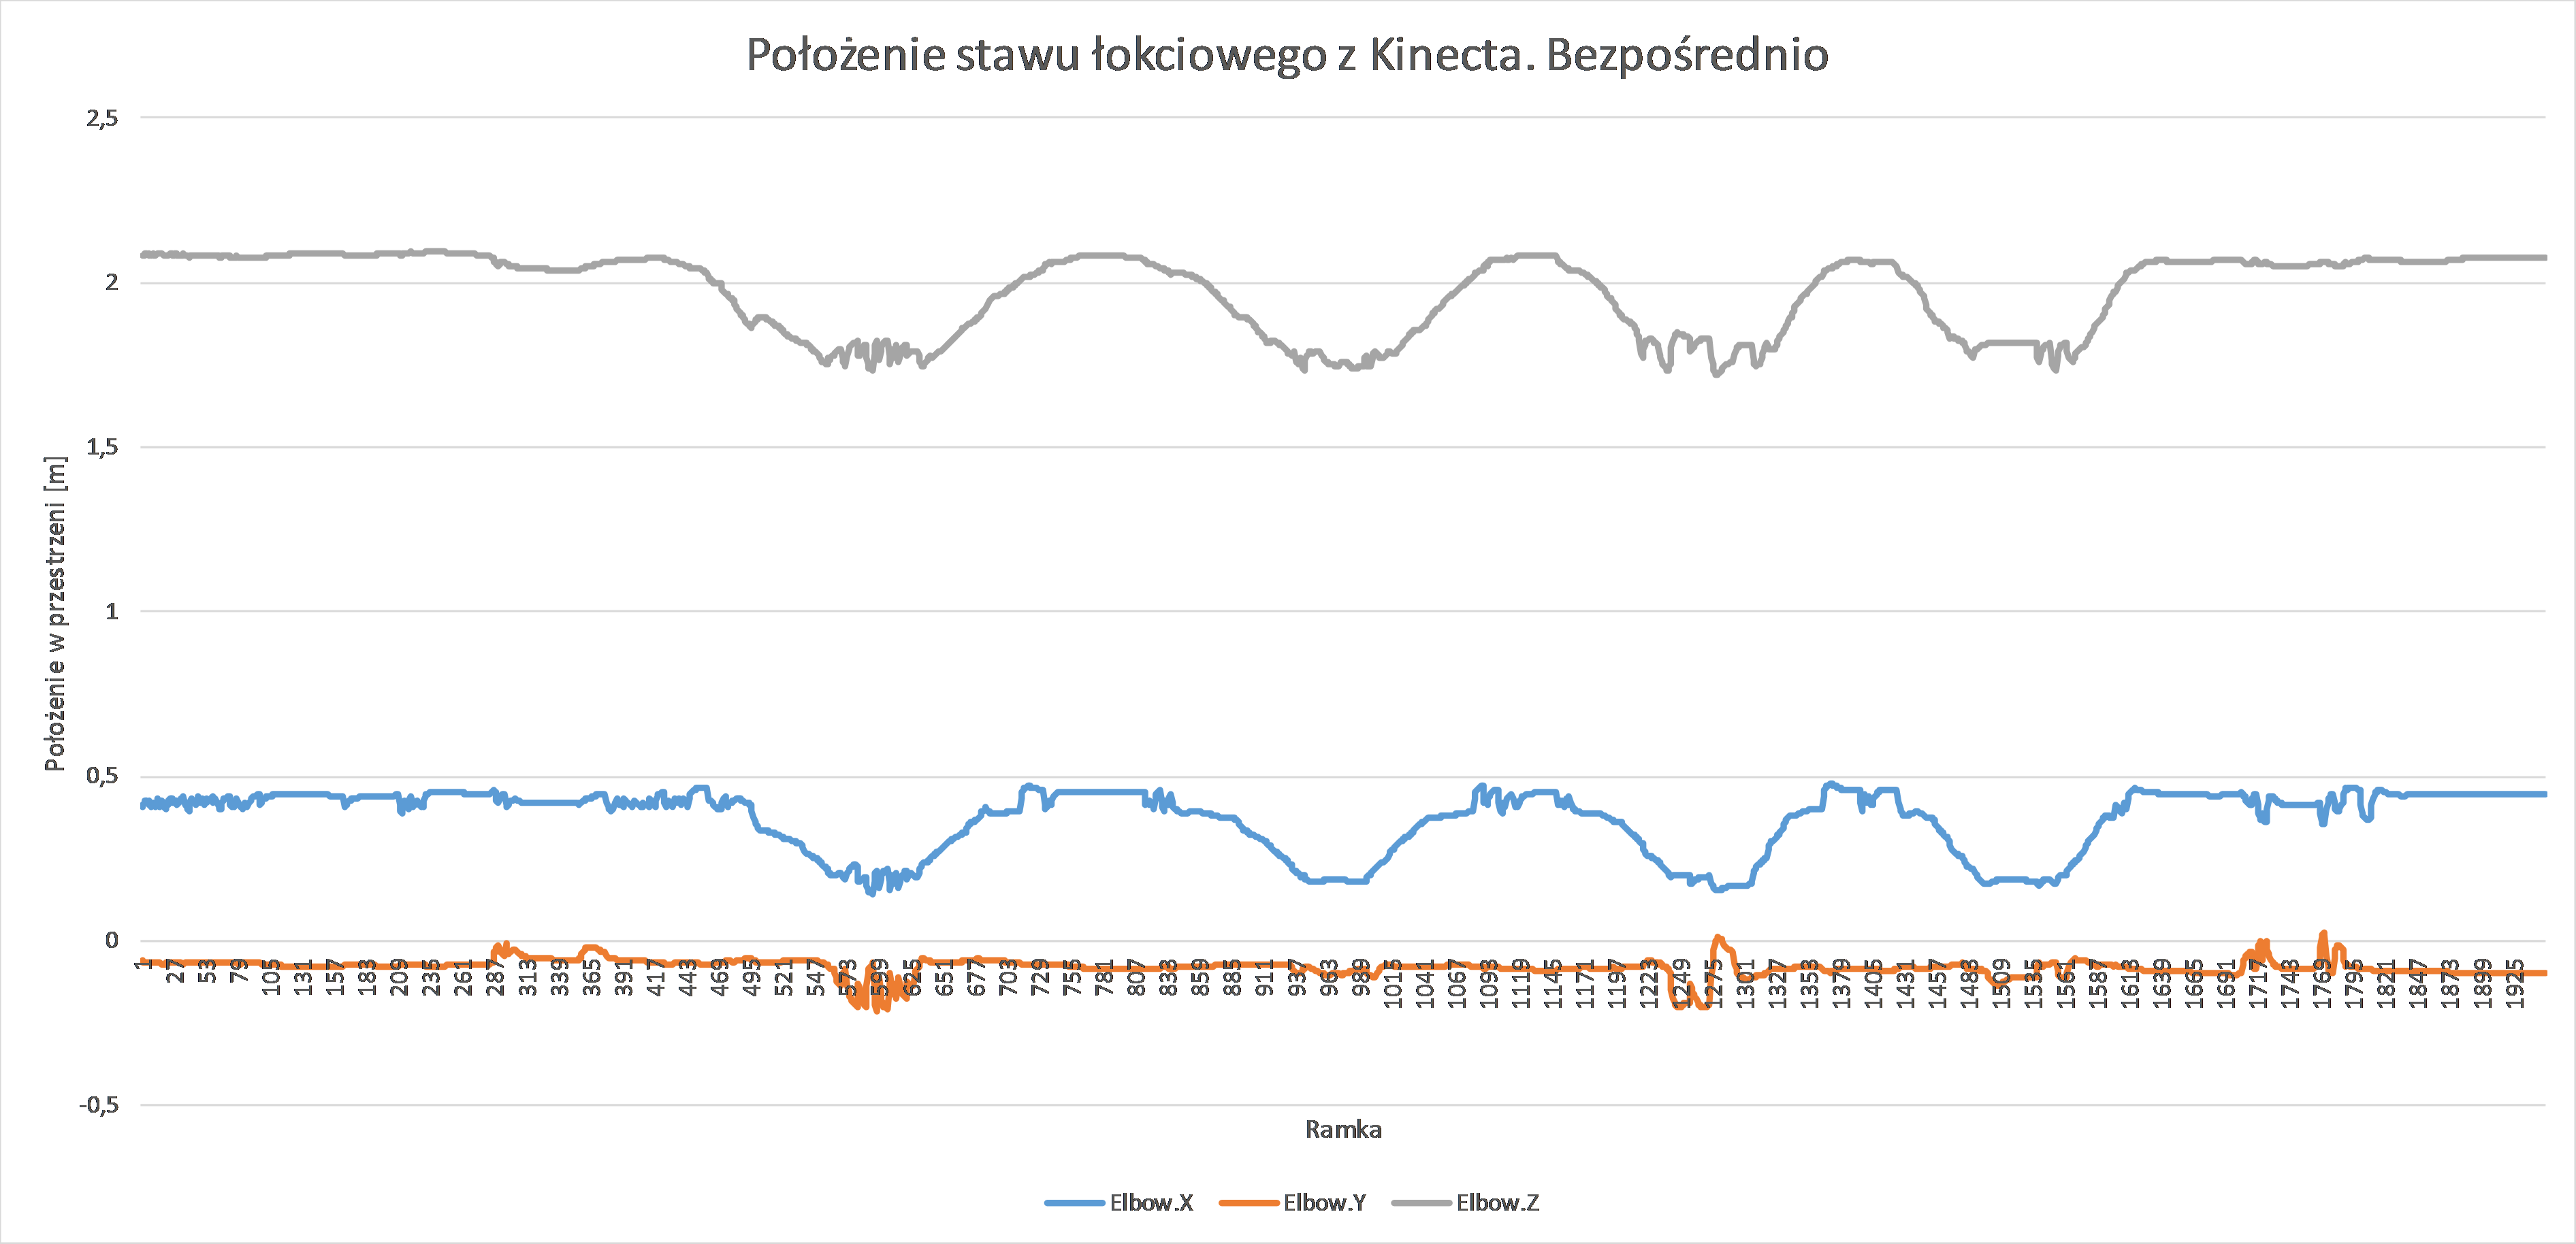
\includegraphics[width=\textwidth]{images/kinectElbowRaw.png}
	}
			
	\subfigure[Pomiar odszumiony]{
		\label{fig:hybrid:kinect:denoised}
		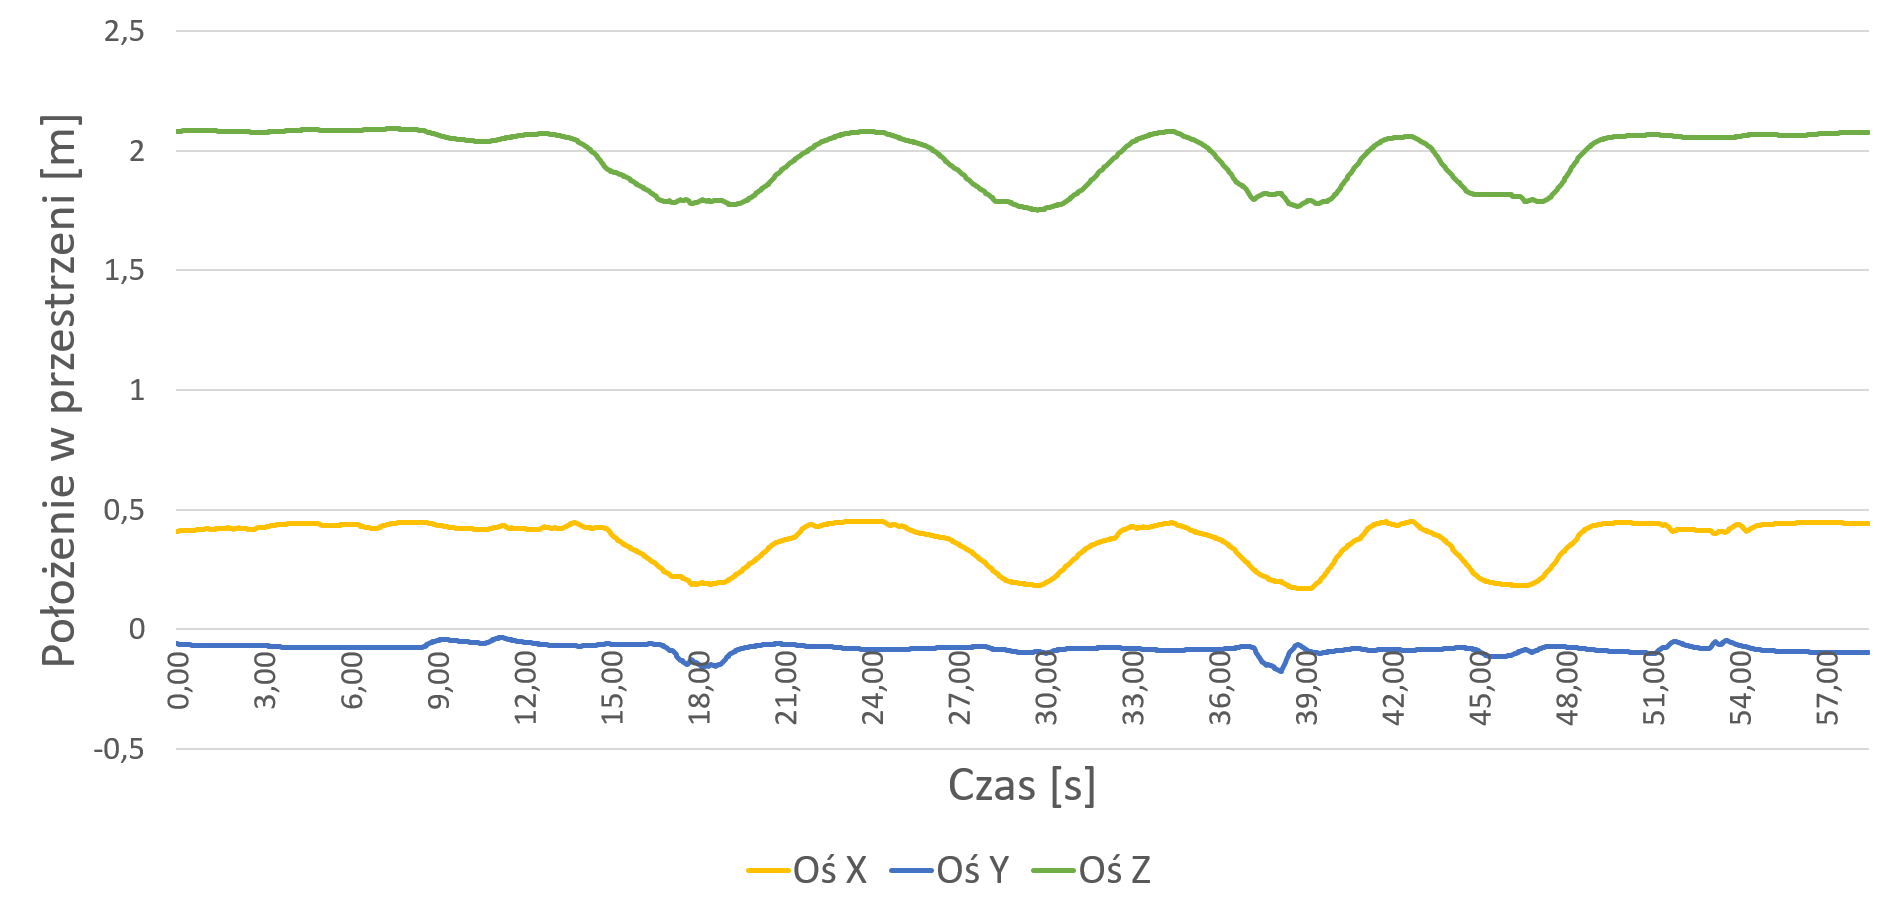
\includegraphics[width=\textwidth]{images/kinectElbowFiltered.png}	
	}
			
	\caption{Wykres przedstawiający oszacowanie położenia stawu łokciowego za pomocą kontrolera Kinect}
\end{figure}

Wartość współczynnika filtracji $\alpha$ została wyznaczona w drodze prowadzonych badań własnych i została ustalona na $0.065$. Przeprowadzony przeze mnie eksperyment (jedno zdanie na czym polegał eksperyment) badający wpływ wartości współczynnika filtracji na dokładność oszacowania pozycji stawów za pomocą kontrolera Kinect polegał na wyznaczeniu średniego błędu oszacowania pozycji stawów między kontrolerem Kinect a danymi referencyjnymi uzyskanymi z systemu śledzenia ruchu firmy Vicon. Rysunek \ref{fig:hybrid:kinect:lpf} przedstawia wykres zależoności uzyskanego średniego błędu oszacowania pozycji stawów w zależności od wartości współczynnika filtracji $\alpha$.

\begin{figure}[!htb]
	\centering 
	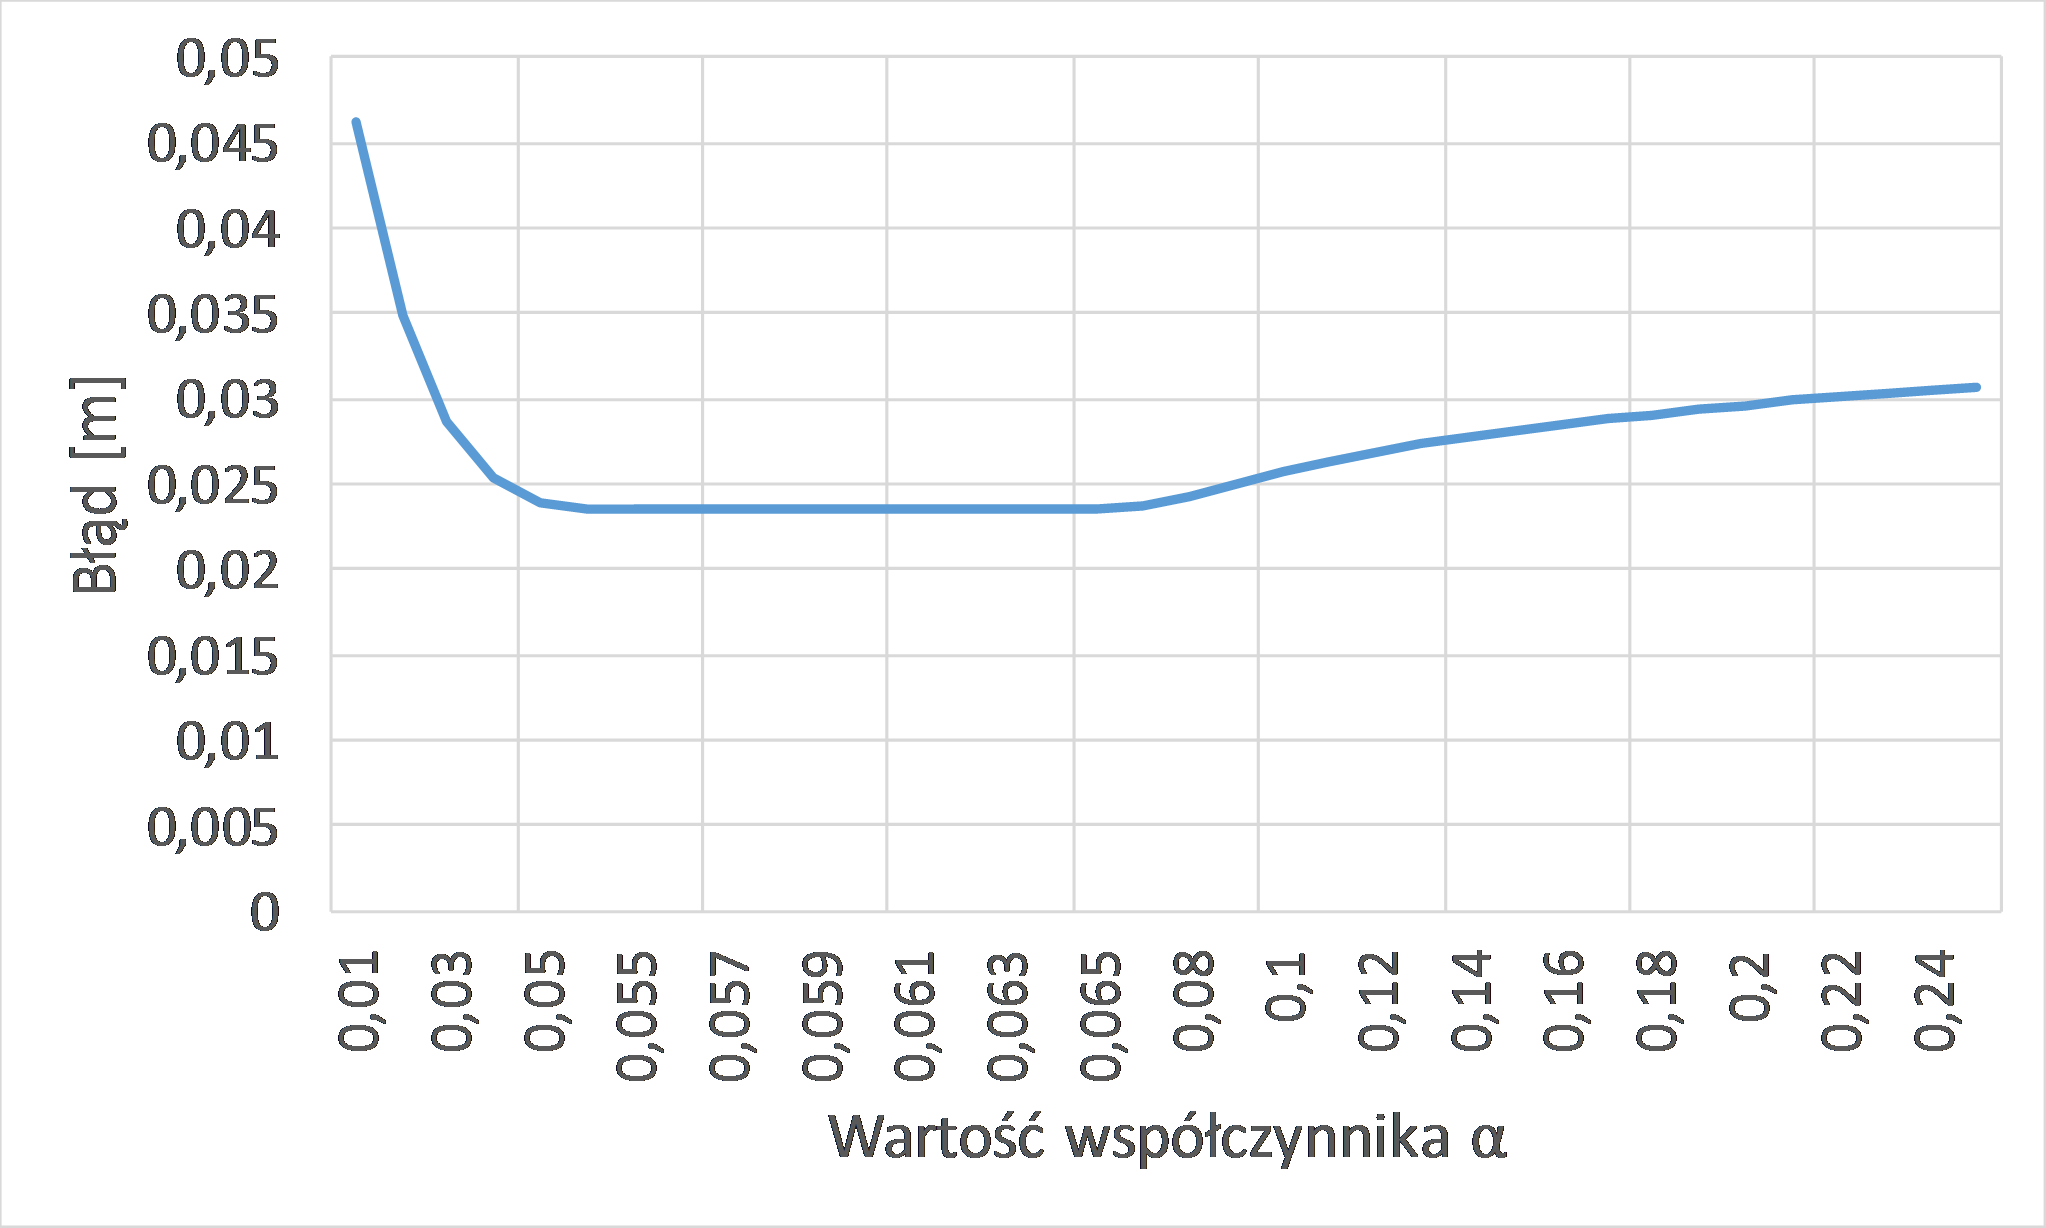
\includegraphics[width=0.75\textwidth]{images/kinectPosErrorAlpha.png}
	\caption{Wykres przedstawiający średni błąd pozycjonowania stawów za pomocą kontrolera Kinect w zależności od współczynnika filtracji $\alpha$}
	\label{fig:hybrid:kinect:lpf}
\end{figure}

Korekcie muszą zostać poddane także oszacowania odległości, w jakiej znajdują się wybrane stawy od kontrolera Kinect. Zgodnie ze wzorami \eqref{eq:characteristics:kinect:distanceAccuracyPoly} i \eqref{eq:characteristics:kinect:distanceAccuracyCoef} definiującymi model błędu szacowania odległości pomiędzy osobą, której ruch jest śledzony a Kinectem, funkcja korygująca ten błąd przybiera postać wzoru \eqref{eq:distCorr}, gdzie wartość $x$ to wartość podlegająca korekcie (oszacowanie odległości) a $y$ to wartość skorygowana (trzeba napisać, ze jest ona wynikiem Twoich badań i jedno zdanie na czym polegały, albo gdzie można znaleźć więcej informacji).
%nie wiem czy x i y to nie jest zły wybór bo te oznaczenia sa dosyć popularne a odległośc kojarzy się bardziej ze zmienną z lub jakąs inną
\begin{equation}
	y = -0.02x^3 + 0.11x^2 - 0.27x + 0.25
	\label{eq:distCorr}
\end{equation}
 

\section{Synchronizacja czasowa}

Aby dane reprezentujące położenie badanego stawu na podstawie czujników inercyjnych oraz kontrolera Kinect mogły być poprawnie złączone, powinny zostać najpierw zsynchronizowane w czasie. Jest to proces, który powinien zostać przeprowadzony przed każdą sesją śledzenia ruchu, np. przed konkretną sekwencją ćwiczeń do wykonania. Synchronizacja czasowa ma na celu określenie przesunięcia czasowego jakie występuje pomiędzy oszacowaniami położenia tych samych stawów w trakcie tego samego ruchu za pomocą każdego z urządzeń pomiarowych osobno (czujników inercyjnych i kontrolera Kinect). Do wyznaczenia przesunięcia czasowego pomiędzy sygnałem uzyskiwanym z czujników inercyjnych ($i(t)$) a tym z kontrolera Kinect ($k(t)$) wykorzystywany został algorytm korelacji wzajemnej (\emph{ang. cross--correlation}) określony wzorem \eqref{eq:cross-cor:1}. Parametr $\tau$ odpowiada za opóźnienie jednego sygnału względem drugiego. Aby wyznaczyć jakie jest przesunięcie czasowe ($d$) pomiędzy dwoma sygnałami należy znaleźć taką wartość argumentu $\tau$ dla którego wartość funkcji korelacji wzajemnej pomiędzy badanymi sygnałami jest największa (wzór \eqref{eq:cross-cor:2}). Aby można było skutecznie wyznaczyć tę wartość, oba sygnały muszą posiadać tę samą częstotliwość próbkowania. Spełnienie tego warunku uzyskano poprzez obniżenie częstotliwości próbkowania sygnału uzyskanego z czujników inercyjnych ze 100Hz  do 30Hz t.j. została ona zrównana do tej, z jaką pracuje Kinect. Pomiary z czujników inercyjnych są buforowane i gdy zostanie pobrany pakiet danych (nie leży mi słowo ramka. Pomyśl nad pakietem danych tak jak wpisałem) z Kinecta, zawartość bufora (jakiego bufora?) zostaje poddana filtrowi medianowemu, aby wyeliminować ewentualne zaburzenia pomiarów. 

\begin{subequations}
	\begin{align}
		(i \ast k)(\tau) & = \int_{-\infty}^{+\infty}i(t)k(t+\tau)dt\label{eq:cross-cor:1}   \\
		d                & = \underset{\tau}{argmax}((f \ast g)(\tau))\label{eq:cross-cor:2} 
	\end{align}
	\label{eq:cross-cor}
\end{subequations}

Wyznaczona wartość przesunięcia w czasie pomiędzy sygnałami $d$ wykorzystywana jest następnie do modyfikacji wartości znacznika określającego czas odebrania danych z czujnika inercyjnego przez komputer PC. Tak zmodyfikowany znacznik czasu wykorzystywany jest do wyznaczenia pomiarów z czujników inercyjnych odpowiadających pomiarom uzyskanym z kontrolera Kinect. Metoda określająca odpowiadające sobie pomiary z kilku sygnałów na podstawie czasów otrzymania wartości każdego z badanych sygnałów nazywana jest decymacją (jakaś referencja?). Przyjmując, że $t_k$ jest znacznikiem czasowym otrzymania na komputerze PC danych z kontrolera Kinect, a $t_i()$ to znaczniki czasowe danych  otrzymanych z czujników inercyjnych i umieszczonych w buforze, wówczas wybór próbki danych pomiarowych z czujników inercyjnych skorelowanych z danymi z kontrolera Kinect wyrażony jest wzorem \eqref{eq:dec}, gdzie $i_{res}$ to numer próbki umieszczonej w buforze danych (nie rozumiem kiedy co i jak jest umieszczane w buforze).

\begin{equation}
	i_{res} = \underset{i}{argmin}(|t_k-(t_i(i) + d)|)
	\label{eq:dec}
\end{equation}

W trakcie prowadzonych autorskich prac badawczych oprócz wyznaczenia przesunięcia czasowego pomiędzy czujnikami inercyjnymi, a kontrolerem Kinect, zostało zbadane przesunięcie czasowe pomiędzy tymi urządzeniami pomiarowymi, a systemem śledzenia ruchu Vicon. Przyjmując, że Vicon działa w czasie rzeczywistym, przesunięcia te określają de facto jakie jest opóźnienie między IMU i Kinectem a rzeczywistym ruchem. I tak, średnie przesunięcie czasowe pomiędzy czujnikami inercyjnymi a systemem Vicon wyniosło około $0.04s$ natomiast pomiędzy Kinectem a systemem Vicon to około $0.09s$. Korelacja wyznaczona między czujnikami inercyjnymi a kontrolerem Kinect wskazuje na średnie przesunięcie szacowania pozycji na koło $0.06s$. (czy skoro wszystko jest równane do Kinecta to to przesunięcie nie powinno być 0.09?)

\section{Łączenie danych}

Strumienie danych pochodzące z poszczegółnych sensorów, zsynchronizowane czasowo oraz poddane filtracji mogą zostać połączone celem uzyskania wypadkowych wartości, lepiej odzwierciedlających układ szkieletu śledzonej postaci. Na tym etapie, prezentowana metoda opiera się na informacji o orientacji przestrzennej poszczególnych kości zamiast na położeniu konkretnych stawów. Podyktowane jest to tym, że w przypadku czujników inercyjnych, wyznaczenie położenia stawów wymaga połączenia informacji o orientacji przestrzennej czujników z modelem szkieletowym zawierającym informację o długościach poszczególnych kości. W przypadku błędnego lub nie dokładnego pomiaru długości kości można spodziewać się błędów w oszacowaniu położenia poszczególnych stawów. Co więcej, ze względu na hierarchiczną budowę modelu szkieletowego, ewentualne błędy wynikające z braku dokładnych pomiarów długości poszczególnych kości szkieletu będą się kumulowały. 
Wykorzystanie położenia stawów szkieltu w procesie łączenia sygnałów z obu źródeł dodatkowo utrudnia fakt niedokładności w oszacowaniu modelu szkieletowego za pomocą kontrolera Kinect. Model ten nie ma zdefiniowanych długości poszczególnych kości na stałe (choćby na czas pojedynczej sesji śledzenia) i są one determinowane przez oszacowanie położenia kolejnych stawów, obarczonych zauważalną zmiennością w czasie. To z kolei skutkuje tym, że długości poszczególnych kości modelu szkieletowego, oszacowanego przez kontroler Kinect, różnią się nawet o kilka $cm$ pomiędzy kolejnymi pomiarami (znowu usunąłem klatki).\\


Dane z obu źródeł (kontroler Kinect i moduł inercyjny) zawierają informacje o orientacji przestrzennej wyrażone w kwaternionach, jednak dalsze obliczenia mające na celu połączenie tych informacji są bardziej intuicyjne przy reprezentacji w postaci kątów Eulera. Konwersja taka przeprowadzona jest zgodnie ze wzorem \eqref{eq:appx:rot:quatToEuler}, a w jej wyniku wartości obrotów wokół każdej z osi układu współrzędnych (którego?), które składają się na orientację przestrzenną danej kości, są wyrażone bezpośrednio. Informacje o orientacji kości wyznaczone na podstawie danych pomiarowych z czujników inercyjnych oraz kontrolera Kinect są od siebie niezależne oraz zawierają uzupełniające się informacje. Wzajemna niezależność i uzupełnianie się danych umożliwia ich połączenie w sposób komplementarny. Łącząc dane w sposób komplementarny każdej z wartości podlegającej łączeniu ($x_1, x_2,\ldots, x_n$) (dlaczego x skoro łaczone sa kąty?) przypisane zostają wagi ($w_1,w_2,\ldots,w_n$) których suma wynosi $1$, a następnie są one ze sobą sumowane z uwzględnieniem wag określających poziom istotności poszczególnych wartości. Wynik sumowania reprezentuje wartość złączonych danych wejściowych ($x^F$). Łączenie komplementarne dla $n$ źródeł przedstawia wzór \eqref{eq:complementaryFilter}.
%skoro łaczone sa kąty to po co wprowadziać znowu x, który w pracy oznaczał juz chyba wszystko
\begin{equation}
	x^F = \sum_{i=1}^{n}{w_i x_i}
	\label{eq:complementaryFilter}
\end{equation}

%(metody reprezentacji orientacji zostały opisane szerzej w dodatku \ref{chap:orientstionRep}). W przypadku Kinecta, pomimo że otrzymujemy te informacje bezpośrednio z urządzenia, należy wyliczyć je samodzielnie ze względu na wykorzystanie filtru dolnoprzepustowego w stosunku do wybranych, śledzonych stawów, które to może wpłynąć na inne wartości obrotów wokół osi układu współrzędnych niż w przypadku pomiarów bezpośrednich. Przyjmując $P_1$ i $P_2$ za położenie dwóch stawów będących związanymi z tą samą kością, z których $P_1$ jest stawem początkowym czyli leży w hierarchii (rys. \ref{fig:characteristics:kinect:skeleton}) bliżej głowy, obrót takiej kości można wyznaczyć zgodnie ze wzorem \eqref{eq:hybrid:rotationEquation}.
%
%\begin{subequations}
%\begin{align*}
%\vec{\textbf{b}} & = \left(P_{2}.X - P_{1}.X\quad P_{2}.Y - P_{1}.Y\quad P_{2}.Z - P_{1}.Z\right) \\
%\hat{\textbf{b}} & = \frac{\vec{\textbf{b}}}{\norm{\vec{\textbf{b}}}} \\
%\vec{\textbf{l}} & = \left(1\quad 0\quad 0\right) \\
%\vec{\textbf{w}} & = \vec{\textbf{l}} \times \hat{\textbf{b}} \\
%d & =  \vec{\textbf{l}} \cdot \hat{\textbf{b}}\\
%r & = \left(d\quad \vec{\textbf{w}}_X\quad \vec{\textbf{w}}_Y\quad \vec{\textbf{w}}_Z\right)\\
%r.W & = r_W + \norm{r}\\
%\hat{r} & = \frac{r}{\norm{r}}\\
%\end{align*}
%\label{eq:hybrid:rotationEquation}
%\end{subequations}
%\equationset{Obliczanie kwaternionu rotacji pomiędzy dwoma wektorami}
%gdzie:
%\begin{conditions}
%\vec{\textbf{b}} & wektor długości przedstawiający kość łączącą stawy o położeniu $P_1$ i $P_2$, $\vec{\textbf{b}} \in \mathbb{R}^3$   \\
%\hat{\textbf{b}} & wektor kierunkowy, znormalizowany wektor $\vec{\textbf{b}}$, $\hat{\textbf{b}} \in \mathbb{R}^3$ \\
%\vec{\textbf{l}} & wektor kierunkowy reprezentujący położenie początkowe względem którego obliczany	jest obrót, $\vec{\textbf{l}} \in \mathbb{R}^3$ \\
%\times & iloczyn wektorowy \\
%\cdot & iloczyn skalarny  \\
%\hat{r} & znormalizowany kwaternion obrotu pomiędzy $\vec{\textbf{l}}$ a $\hat{\textbf{b}}$, $\hat{r} \in \mathbb{H}$  \\
%\end{conditions}

Prezentowana w niniejszej dysertacji hybrydowa metoda śledzenia ruchu kończyn człowieka łączy ze sobą dane pochodzące z dwóch źródeł. Dane te są w postaci trójelementowych wektorów orientacji $\begin{bmatrix}  \Phi &  \Theta & \Psi \end{bmatrix}$, gdzie każdy z elementów oznacza obrót wokół pojedynczej osi układu współrzędnych. Wektor ten stanowi reprezentację orientacji przestrzennej segmentu szkieletu w postaci kątów Eulera, wyznaczoną przez konwersję kwaternionów otrzymanych na podstawie pomiarów czujników inercyjnych i kontrolera Kinect. Wagi wykorzystywane w procesie łączenia danych są wyznaczane indywidualnie dla każdego z elementów wektora. Przyjmując, że wagi $w_\Phi , w_\Theta , w_\Psi$ oznaczają poziom istotności informacji otrzymanych na podstawie pomiarów czujników inercyjnych ($\begin{bmatrix}  \Phi^I &  \Theta^I &  \Psi^I \end{bmatrix}$) wówczas komplementarne łączenie ich z danymi otrzymanymi z kontrolera Kinect ($\begin{bmatrix}  \Phi^K &  \Theta^K &  \Psi^K \end{bmatrix}$) dla danej chwili $t$ przedstawia wzór \eqref{eq:hybrid:reliableFusion}

\begin{equation}
	\begin{bmatrix}  \Phi^F \\  \Theta^F \\  \Psi^F \end{bmatrix}_t = 
	\begin{bmatrix}  w_\Phi&0&0 \\  0&w_\Theta&0 \\  0&0&w_\Psi \end{bmatrix}
	\begin{bmatrix}  \Phi^I \\  \Theta^I \\  \Psi^I \end{bmatrix}_t + 
	\begin{bmatrix}  1-w_\Phi&0&0 \\  0&1-w_\Theta&0 \\  0&0&1-w_\Psi \end{bmatrix}
	\begin{bmatrix}  \Phi^K \\  \Theta^K \\  \Psi^K \end{bmatrix}_t
	\label{eq:hybrid:reliableFusion}
\end{equation}
% w powyzszych rozwazaniach posługujesz się kątami i to jest zrozumiałe, to po co wczesniej przy łączeniu kompementarnym są ixy?

Wzór \eqref{eq:hybrid:reliableFusion} jest wykorzystywany zawsze wtedy, kiedy dane podlegające łączeniu są dobrej jakości i możemy je uznać za prawidłowe. W takiej sytuacji współczynniki wag $w_\Phi , w_\Theta , w_\Psi$ są wartościami stałymi wynoszącymi odpowiednio $0.98,0.05,0.65$. (skąd te wartości? Podać ich źródło.)\\
Waga $w_\Phi$ odpowiada za obrót wokół osi przechodzącej wzdłuż ciała ($X$) (konieczne odwołanie do rysunkku, który powinien te wszystkie układy i szkielet przedstawić na początku jednoznacznie i potem konsekwentnie stosować). Wysoka wartość tej wagi wynika z faktu, że wartość obrotu wokół tej osi jest mierzalna jedynie przez czujniki inercyjne. Dzięki wadze zbliżonej do wartości $1$, pomiary uzyskane z Kinecta są niemal ignorowane.\\
$w_\Theta$ jest wagą określająca istotność informacji o obrocie wokół osi zgodnej z kierunkiem działania grawitacji ($Z$) (równiez odwołanie do rysunku j.w.). Wartość tego obrotu jest bardziej wiarygodnie i stabilnie w czasie szacowana przez kontroler Kinect. Niska wartość wagi $w_\Theta$ zmniejsza wpływ danych wyznaczonych na podstawie pomiarów czujników inercyjnych (obarczonych znaczącym dryfem) na wartości wypadkowe będące wynikiem łączenia danych.\\ 
Waga $w_\Psi$ określa poziom istotności informacji o obrocie wokół osi skierowanej w stronę obserwacji kontrolera Kinect (rysunek j.w.). Obrót ten jest szacowany zarówno przez kontroler Kinect jak i na podstawie pomiarów z czujników inercyjnych. Oszacowania te mają jednak różną dokładność i różnica ta jest odzwierciedlona w przyjętej (empirycznie?) wartości wagi. Według badań opublikowanych przez twórcę, wykorzystywanego w niniejszej pracy, filtru Madgwicka \cite{Madgwick2010}, jego metoda wyznaczania orientacji przestrzennej na podstawie pomiarów z czujników inercyjnych zapewnia dokładność około $\pm2\degree$. W badaniach własnych autora dokładność ta była zbliżona do $\pm3\degree$. Z kolei dokładność oszacowania obrotu wokół osi zgodnej z kierunkiem obserwacji (zamiast oś zgodna z kierunkiem obserwacji to podać jej symbol i odwołac się do konkretnego rysunku) kontrolera Kinect przez to właśnie urządzenie, określona na podstawie badań własnych jak i opisów dostępnych w literaturze \cite{Huber2015}, wynosi około $\pm6\degree$. Niemal dwukrotnie większa dokładność (czy mniejszy błąd?) oszacowania obrotu wokół osi $Y$ (tutaj dopiero pojawił się symbol osi) na podstawie pomiarów z czujników inercyjnych ma swoje przełożenie w wartości wagi $w_\Psi$.\\
Rysunek \ref{fig:handAxes} przedstawia układ współrzędnych wraz z obrotami odpowiadającymi każdej z osi tego układu, w odniesieniu do ręki człowieka.

\begin{figure}[!htb]
	\centering	
	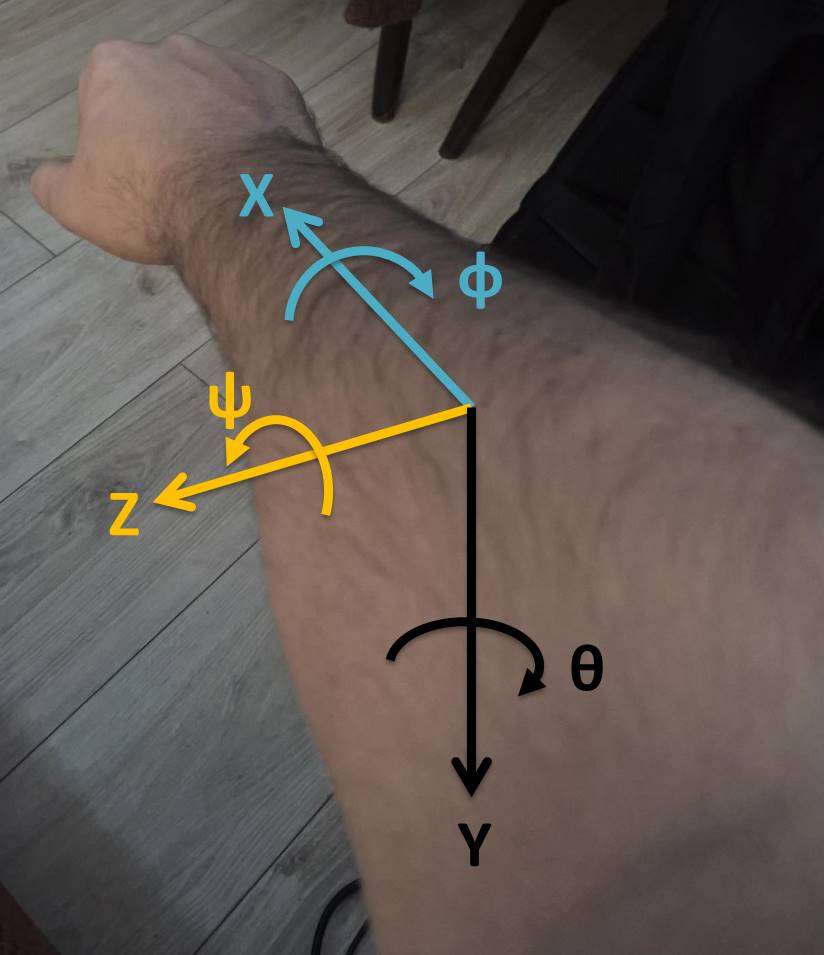
\includegraphics[width=0.5\textwidth]{images/handAxes.jpg}	
	\caption{Odniesienie układu współrzędnych $XYZ$ wraz z obrotami $\Phi , \Theta , \Psi$ do ręki człowieka.}
	\label{fig:handAxes}
\end{figure}
%na rysunku brakuje szerszego kontekstu jak uustawiony jest Kinect i jak sa zdefiniowane pozostałe układy współrzędnych

Określenie czy oszacowania kątów uzyskane za pomocą kontrolera Kinect są wystarczającej jakości do łączenia ich z oszacowaniami kątów uzyskanymi z czujników inercyjnych wykonywane jest każdorazowo na podstawie kryteriów związanych z realizowanym ruchem. \\
Pierwszym kryterium branym pod uwagę jest obrót całej sylwetki względem kamery, liczony jako kąt pomiędzy linią barków a kamerą w płaszczyźnie $X$--$Z$ (znowu brakuje rysunku z szerszym kontekstem) zgodnie ze wzorem \eqref{eq:characteristics:kinect:bodyRotationAngle}. Na podstawie zbadanych wcześniej charakterystyk obu urządzeń wiadomo, że dane które można wiarygodnie wykorzystać do łączenia są możliwe do uzyskania tylko gdy sylwetka nie jest obrócona o więcej niż $50\degree$. Oprócz wartości kąta obrotu sylwetki brane jest także pod uwagę odchylenie standardowe estymacji tego obrotu. Przyjmując, że $X$ (dlaczego znowu x przecież kąty majhą swoje oznaczenia może chociaż alfa?) to zbiór wartości oszacowań kąta obrotu sylwetki z ostatnich $3s$ (ok. 90 elementów w zbiorze) a $\bar{X}$ to średnia arytmetyczna elementów w tym zbiorze, wówczas odchylenie standardowe $\sigma$ definiuje wzór \eqref{eq:stdDev}.

\begin{equation}
	\sigma = \sqrt{\frac{\sum_{i=1}^{n}{(X_i - \bar{X})^2}}{n-1}}
	\label{eq:stdDev}
\end{equation}

Branie pod uwagę zarówno bezwzględnej wartości estymacji obrotu sylwetki (nie wiem gdzie ta wartośc bezwzględna występuje? gdzie jest kryterium?) wraz z odchyleniem standardowym uzyskiwanych oszacowań spowodowane jest faktem, że w momencie wystąpienia okluzji jednego lub obu stawów barkowych i błędów oszacowania ich położenia następuje błędne oszacowanie wartości obrotu. W praktyce oznacza to, że wyznaczony kąt obrotu sylwetki może przyjąć dowolną wartość. Przykład szacowania kąta obrotu sylwetki względem kontrolera Kinect przedstawia wykres \ref{fig:hybrid:kinect:kinectRotationVariance}. W trakcie tego eksperymentu badawczego wykonywany był obrót postaci względem kontrolera Kinect do kąta $90\degree$ i powrót do pozycji równoległej do urządzenia pomiarowego, czyli do kąta $0\degree$. Przy obrocie sylwetki nie przekraczającym $50\degree$ odchylenie standardowe oszacowań z przyjętego okresu czasu nie przekracza wartości $1.5\degree$. W związku z tym w opisywanej w niniejszej dysertacji hybrydowej metodzie śledzenia ruchu kończyn człowieka, autor przyjął, że śledzona postać nie jest obrócona za bardzo w stosunku do kontrolera Kinect jeśli oszacowanie jego kąta obrotu jest $\le 50\degree$ przy odchyleniu standardowym $\le 1.5 \degree$.

\begin{figure}[!htp]
	\centering
			
	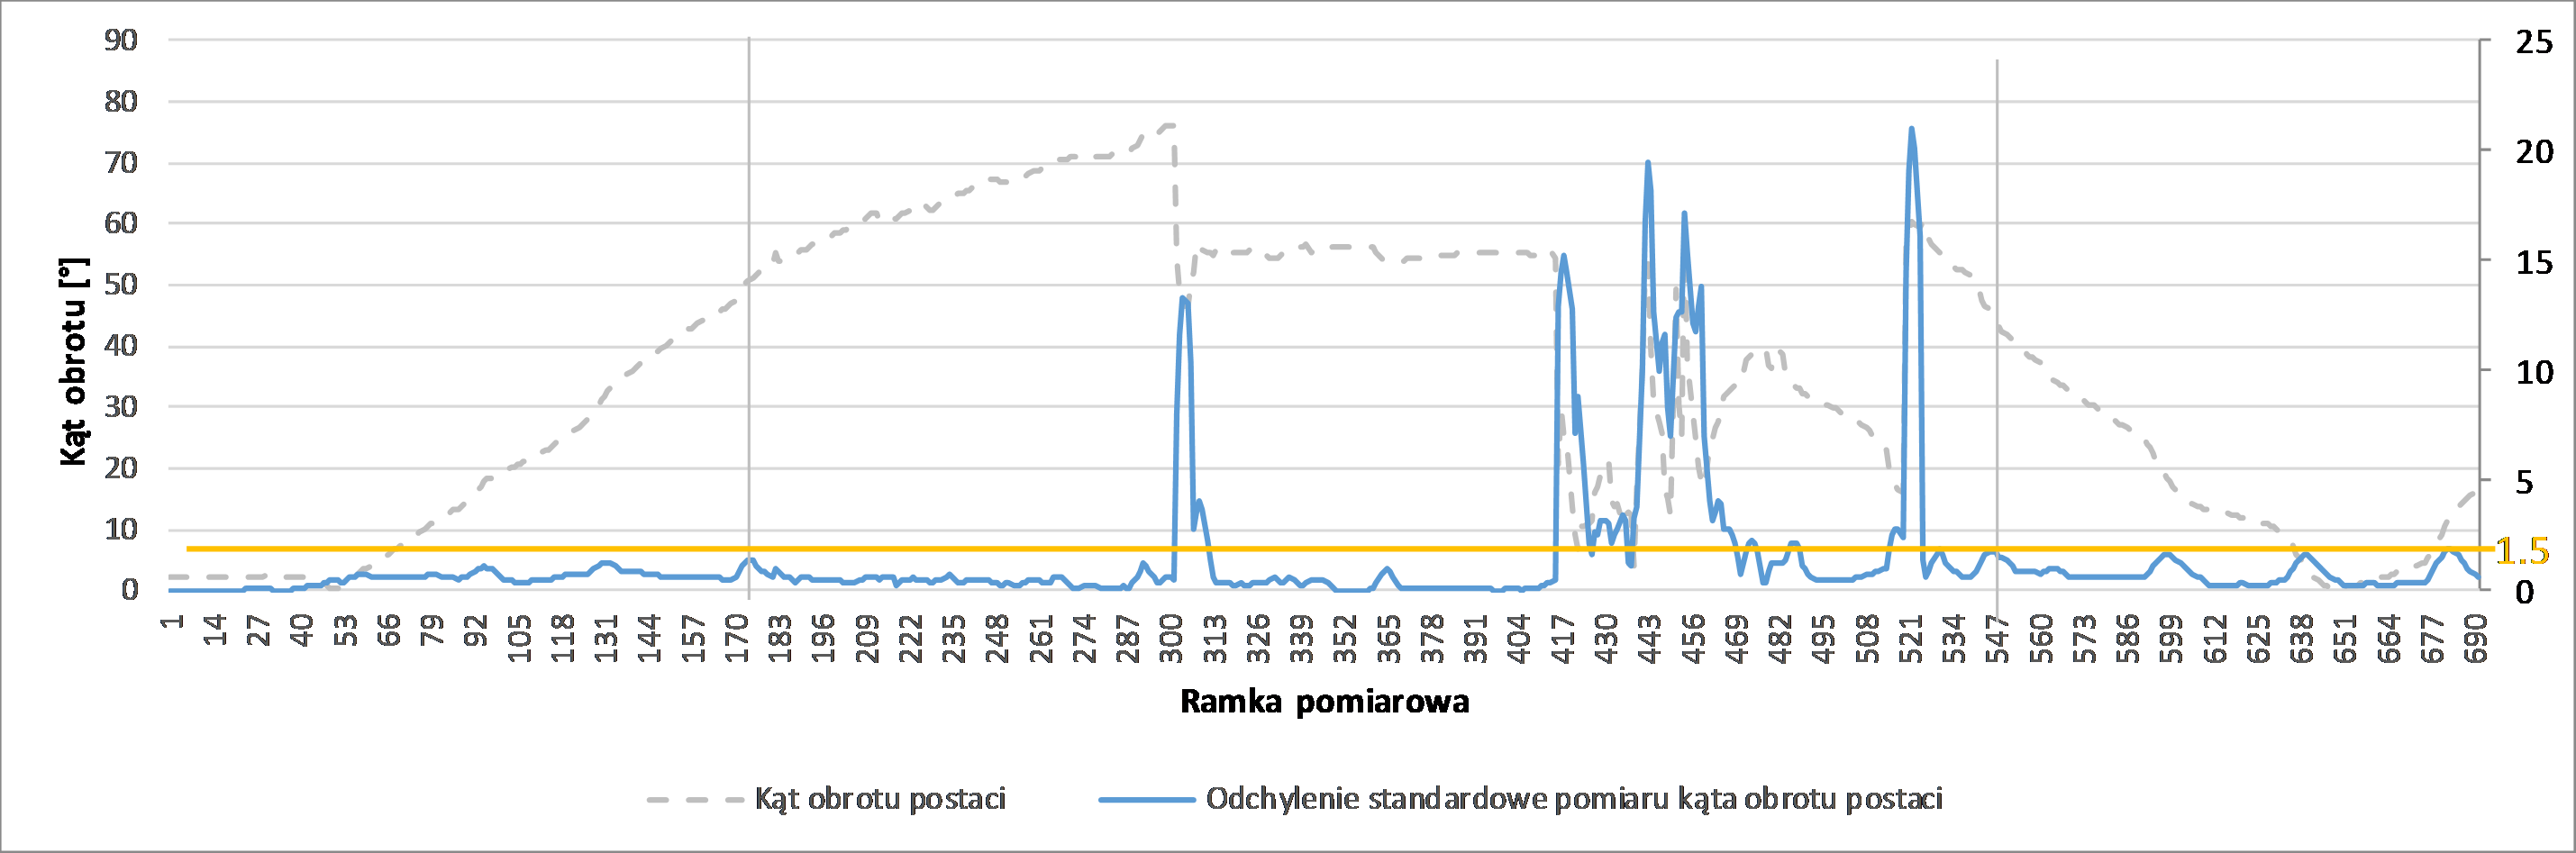
\includegraphics[width=0.75\textwidth]{images/kinectRotationStdDev.png}
	\caption{Odchylenie standardowe estymacji kąta obrotu postaci względem Kinecta}
		
	\label{fig:hybrid:kinect:kinectRotationVariance}
\end{figure}

Oprócz obrotu całej postaci, ocenie podlega także stabilność pomiarów samych stawów. Pierwszym parametrem jaki brany jest pod uwagę jest stan śledzenia poszczególnych stawów, który może przyjąć jedną z 3 wartości opisanych szerzej w podrozdziale \ref{ssec:characteristics:kinect:limitation}. Wartość \emph{NotTracked} jest od razu traktowana jako wskazanie, że dane związane z danym stawem (jego pozycja, ale także orientacja kości związanych z nim) są niewiarygodne. W przypadku pozostałych 2 możliwych stanów śledzenia stawu sprawdzany jest poziom szumu za pomocą filtru górnoprzepustowego w postaci \eqref{eq:hybrid:kinect:hpf}. 

\begin{equation}
	n_t = \delta n_{t-1} + \delta(P_t - P_{t-1}) 
	\label{eq:hybrid:kinect:hpf}
\end{equation}

gdzie:
\begin{conditions}
	n_t & poziom szumu w aktualnym pomiarze \\
	n_{t-1} & poziom szumu w poprzednim pomiarze \\
	P_t & położenie stawu w aktualnym pomiarze \\
	P_{t-1} & położenie stawu w poprzednim pomiarze \\
	\delta & współczynnik filtracji  $\delta = 0.01$ \\
\end{conditions}

\begin{figure}[!htb]
	\centering 
	\subfigure[Staw śledzony ze statusem \emph{Tracked}]
	{
		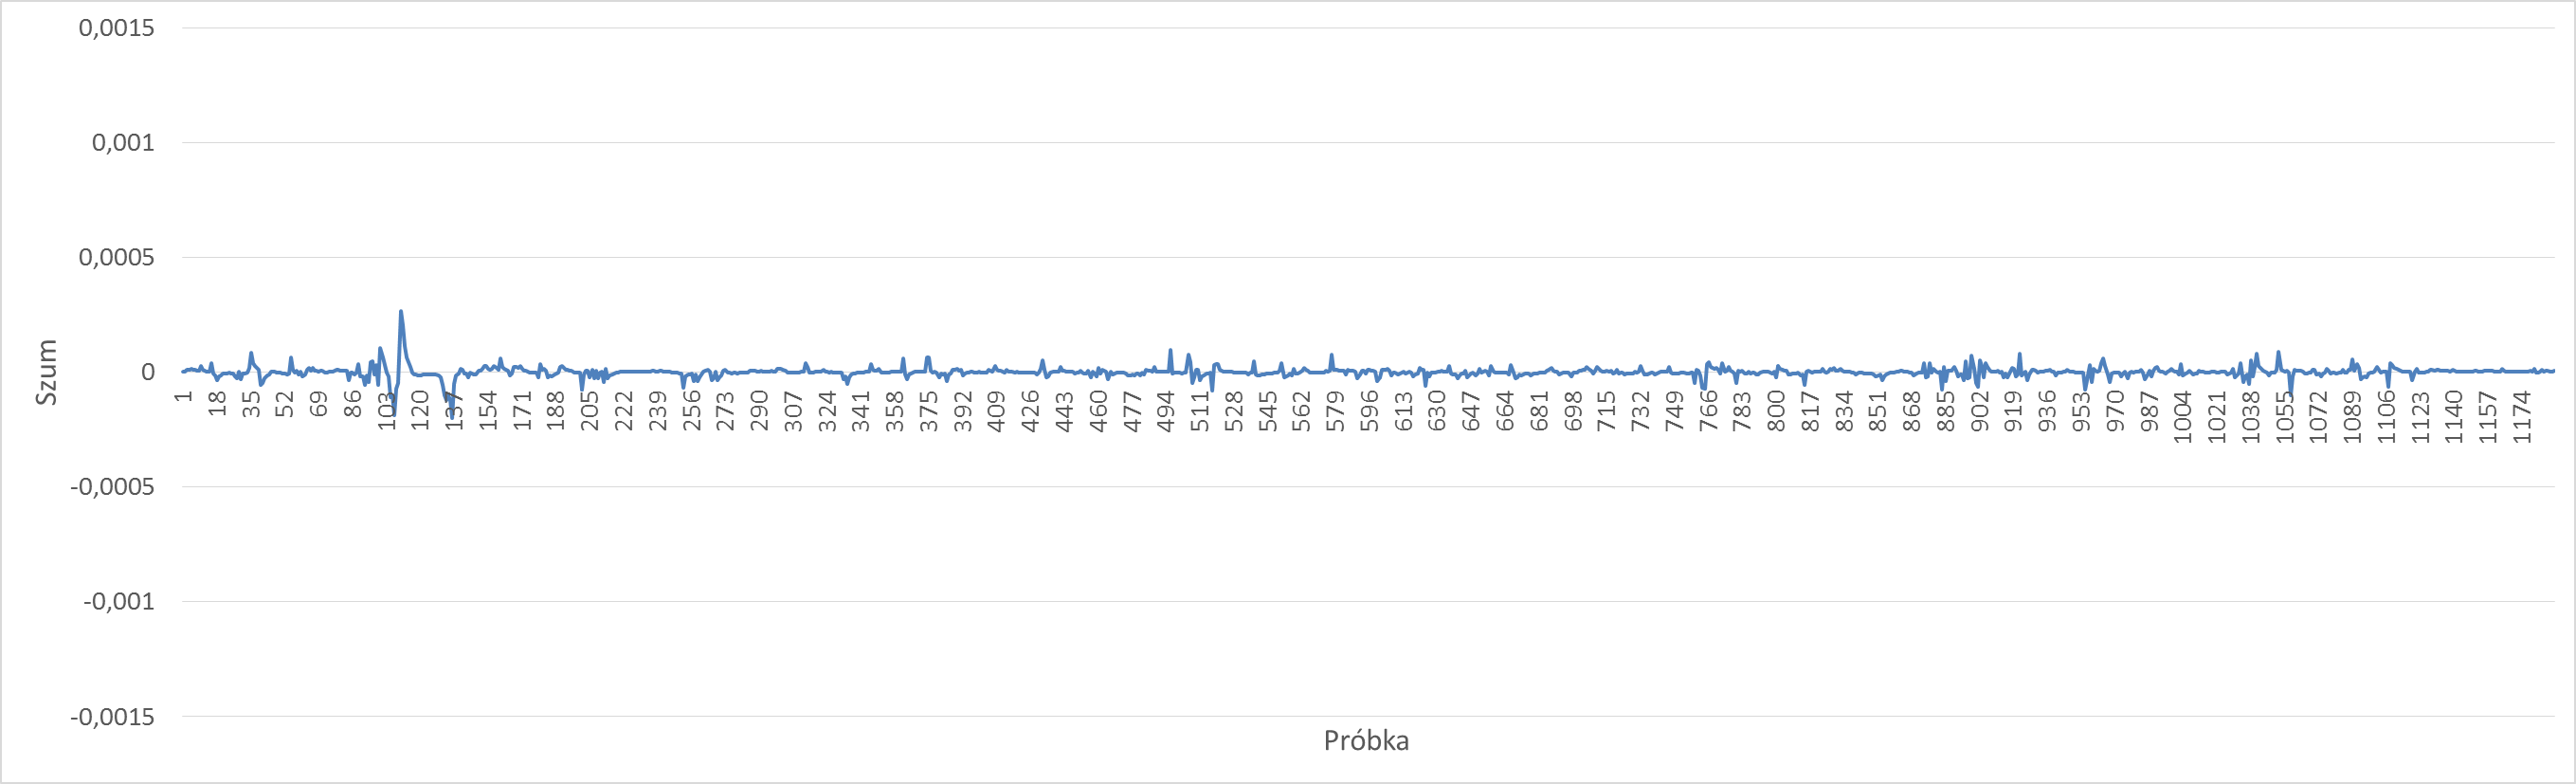
\includegraphics[width=0.75\textwidth]{images/Fig09.png}
		%\vspace{2.5cm}
		\label{fig:hybrid:kinect:hpfNotOccluded}
	}
	\subfigure[Staw śledzony ze statusami \emph{Tracked} i \emph{Interferred}]
	{
		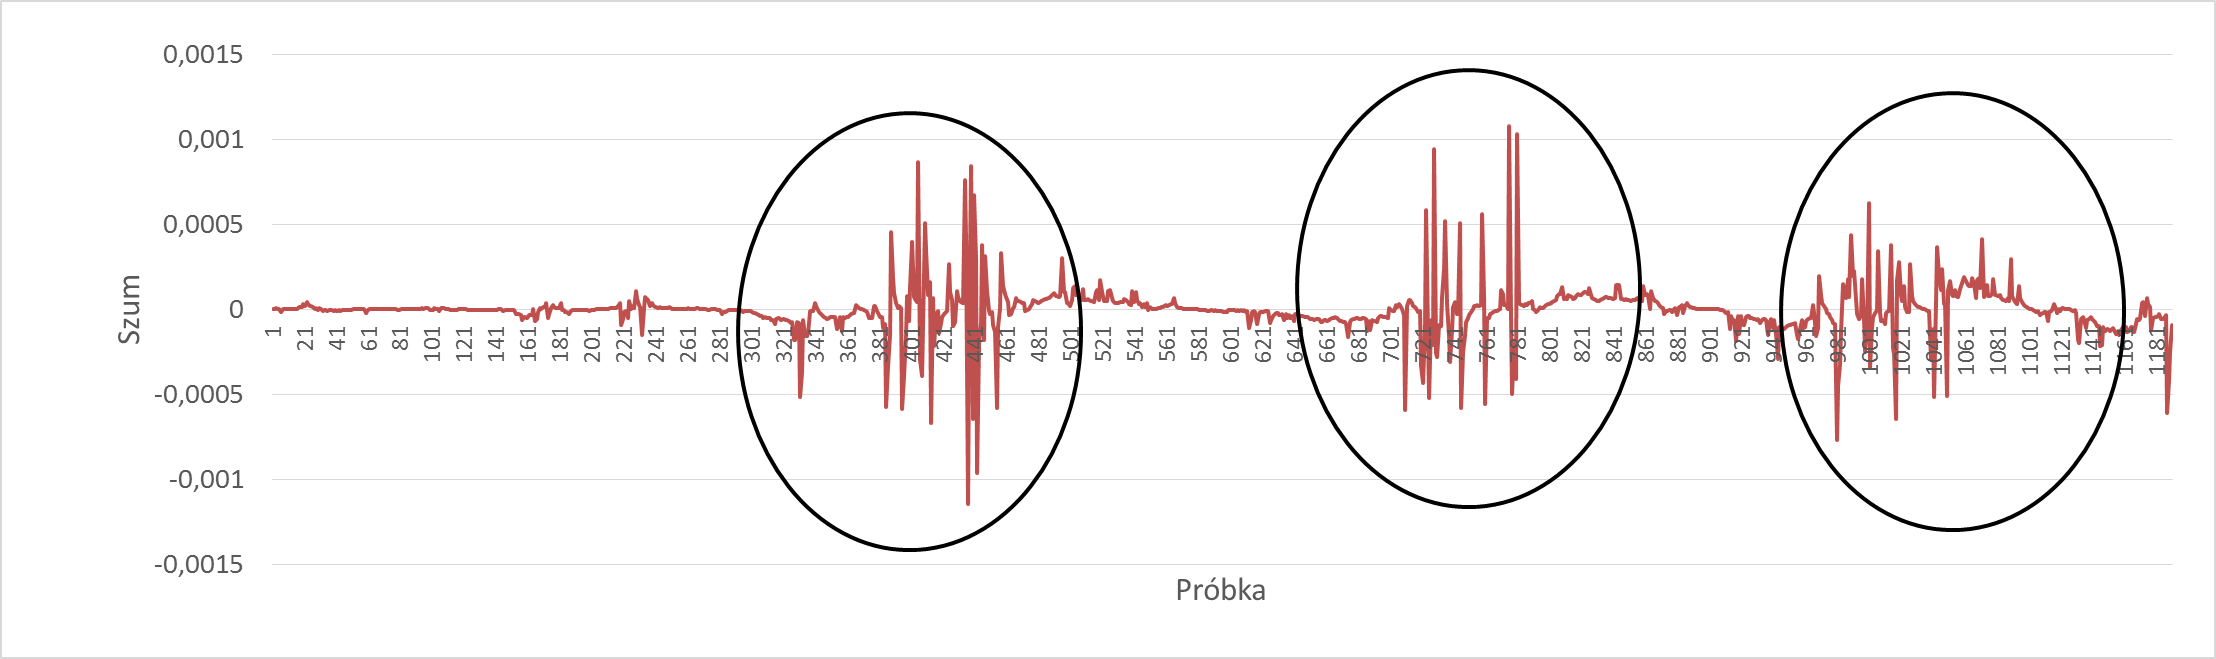
\includegraphics[width=0.75\textwidth]{images/Fig10.png}
		%\vspace{2.5cm}
		\label{fig:hybrid:kinect:hpfOccluded}
	}
	\caption{Wynik działania filtru górnoprzepustowego (wz. \eqref{eq:hybrid:kinect:hpf}) w stosunku do położenia wybranych stawów w przestrzeni w osi $Z$ dla stawu śledozonego ze stałym statusem \emph{Tracked} (a) oraz zmiennym statusem \emph{Tracked} i \emph{Interferred} (b)}
	\label{fig:hybrid:kinect:hpfResults}
\end{figure}

Wykresy \ref{fig:hybrid:kinect:hpfNotOccluded} i \ref{fig:hybrid:kinect:hpfOccluded} przedstawiają wynik działania filtru górnoprzepustowego dla oszacowania położenia stawu nadgarstkowego w przypadku kiedy staw cały czas posiadał status śledzenia \emph{Tracked} oraz kiedy w trakcie wykonywanego ruchu status zmieniał się na \emph{Interferred}. Dla zachowania przejrzystości, wykresy przedstawiają wspomniany wynik dla położenia stawu wyznaczonego wzdłuż jednej z osi. Na wykresie \ref{fig:hybrid:kinect:hpfOccluded} zostały zaznaczone (w jaki sposób zaznaczone?) te miejsca kiedy nastąpiła zmiana statusu śledzenia. Na wspomnianych wykresach widać, że poziom szumu pozostaje niski dla oszacowania położenia stawu kiedy status jego śledzenia przyjmuje wartość \emph{Tracked}. W innym przypadku poziom szumu wzrasta wielokrotnie i utrzymuje się do momentu ponownego przyjęcia statusu  \emph{Tracked}. W wartości oszacowania położenia stawu widoczne jest to w postaci zauważalnego efektu drgania danego stawu. Na podstawie przeprowadzonych badań własnych, w metodzie śledzenia ruchu opisywanej w niniejszej dysertacji jako graniczną wartość zaszumienia danych pomiarowych kontrolera Kinect ($n$), dla których możliwe jest ich łączenie z danymi uzyskanymi z czujników inercyjnych na podstawie wzoru \eqref{eq:hybrid:reliableFusion}, autor przyjął $|n| \le 0.0004$\\

W przypadku, kiedy położenie stawów wyznaczone przez kontroler Kinect nie może być uznane za wiarygodne (zazwyczaj spowodowane jest to okluzją, \ref{ssec:characteristics:kinect:limitation}), równanie \eqref{eq:hybrid:reliableFusion} ulega modyfikacji i przyjmuje postać jak w \eqref{eq:hybrid:unreliableFusion} 

\begin{equation}
	\label{eq:hybrid:unreliableFusion}
	\begin{bmatrix}  \Phi^F \\  \Theta^F \\  \Psi^F \end{bmatrix}_t = 
	\begin{bmatrix}  \Phi^F \\  \Theta^F \\  \Psi^F \end{bmatrix}_{t-1} + 
	\begin{bmatrix}  w_\Phi&0&0 \\  0&w_\Theta&0 \\  0&0&w_\Psi \end{bmatrix}
	(\begin{bmatrix}  \Phi^I \\  \Theta^I \\  \Psi^I \end{bmatrix}_t -
	\begin{bmatrix}  \Phi^I \\  \Theta^I \\  \Psi^I \end{bmatrix}_{t-1})
\end{equation}

W tym przypadku zmianie ulegają wartości części wag z jakimi zostają połączone dane. O ile wartość $w_\Phi$ nie ulega zmianie i wynosi $0.98$, o tyle pozostałe dwie wagi są zależne od czasu i wyrażają się wzorem \ref{eq:dynamicWeight}.
\begin{equation}
	w_{\Theta,\Psi} = f(t_{szum}) = (1-\frac{t_{szum}}{10}) * 0.65
	\label{eq:dynamicWeight}
\end{equation}

Wartość $t_{szum}$ oznacza czas trwania okresu niepewności pomiarów. Jeśli czas, w którym utrzymuje się niepewność pomiarów kontrolera Kinect przekracza $10s$ wówczas wartość $t_{szum}$ pozostaje przy wartości $10$. Skutkuje to tym, że po upływie tego czasu, orientacja przestrzenna poszczególnych kości, a co za tym idzie położenie stawów, nie będzie aktualizowane za wyjątkiem obrotu wokół własnej osi ($kąt \Phi$). \\

\begin{savenotes}
	\begin{figure}[hbp]
		\centering
		\begin{tikzpicture}[
				auto,
				block/.style    = { rectangle, draw=blue, thick, 
					fill=white, text width=50, text centered,
					minimum height=2em, font=\tiny },
				newBlock/.style    = { rectangle, draw=green, thick, 
					fill=green!20, text width=55, text centered,
					minimum height=2em, font=\tiny }
			]
																													
			\node[block](IMU)at (-1,2){Czujniki inercyjne};
			\node[newBlock](Temp) at (2,0.5){Korekta \\ względem \\ temperatury (wz. \eqref{eq:hybrid:temperatureCorrection})};
			\node[block](AHRS) at (4.5,2){Filtr \\ Madgwicka + LERP};
			\node[block](EulerImu) at (7,2){Transformacja do \\ kątów Eulera (wz. \eqref{eq:appx:rot:quatToEuler})};
			\node[newBlock](Fusion) at (7, 0){Łączenie \\ orientacji (wz. \eqref{eq:hybrid:reliableFusion} i~\eqref{eq:hybrid:unreliableFusion})};
			\node[block](EulerKinect) at (7,-2){Transformacja do \\ kątów Eulera (wz. \eqref{eq:appx:rot:quatToEuler})};
			\node[newBlock](Triage) at (7,-3.5){Ocena jakości pomiarów Kinecta};
																													
																													
			\node[newBlock](LPF) at (4.5,-3.5){Filtr \\ dolnoprzepustowy (wz. \eqref{eq:hybrid:kinect:lpf})};
			\node[newBlock](Distance) at (2,-3.5){Korekta \\ odległości (wz. \eqref{eq:distCorr})};
			\node[block](Kinect)at (-1,-3.5){Kinect};
																													
			\node[block](quat) at (11.5,0){Transformacja do \\ kwaternionu (wz. \eqref{eq:appx:rot:eulerToQuat})};
			\node[block](pos) at (11.5,-3.5){Wyznaczenie pozycji stawu};
																													
			\draw[->]  (Kinect) -- node[above,font=\tiny]{P} ++ (Distance);
			\draw[->]  (Distance) --  node[above,font=\tiny]{P'} ++(LPF);
			\draw[->]  (LPF) -- (Triage);
			\draw[->]  (Triage) -- (EulerKinect);
			\draw[->]  (EulerKinect) -- node[left,font=\tiny]{$\begin{bmatrix}  \Phi^K  \Theta^K  \Psi^K \end{bmatrix}$} ++(Fusion);
																													
																													
																													
			\draw[->]  (Fusion) -- node[above,font=\tiny]{$\begin{bmatrix}  \Phi^F  \Theta^F  \Psi^F \end{bmatrix}$} ++ (quat);
			\draw[->]  (quat) -- node[left,font=\tiny]{$Q^F$}++(pos);
			\draw[->]  (EulerImu) --  node[left,font=\tiny]{$\begin{bmatrix}  \Phi^I  \Theta^I  \Psi^I \end{bmatrix}$} ++ (Fusion);
			\draw[->]  (AHRS) --  node[above,font=\tiny]{$Q^I$} ++ (EulerImu);
			\draw[->]  (Temp) -| node[below,font=\tiny]{A'}  (AHRS);
			\draw[->]  (IMU) -- node[above,font=\tiny]{G} ++ (AHRS);
			\draw[->]  (0, 1.8) -|  node[right,font=\tiny]{T} ++ (Temp);
			\draw[->]  (IMU) |-  node[below,font=\tiny]{A}  (Temp);
			\draw[dashed, ->](quat) -- (11.5,3.0) node[above,font=\tiny]{$Q^F$} -|  (AHRS);
			\draw[->]  (pos) -- node[left,font=\tiny]{$\left[p_x^F,p_y^F,p_z^F\right]$} (11.5,-4.5);
		\end{tikzpicture}
		\caption{Diagram przedstawiający kolejne etapy działania autorskiej metody łączenia danych IMU i~Kinecta.}
																
		\label{fig:hybrid:methodDiagram}
	\end{figure}
\end{savenotes}
Poszczególne etapy metody opisanej powyżej przedstawione są na diagramie z rysunku \ref{fig:hybrid:methodDiagram} i odzwierciedlają kroki opisane w niniejszym rozdziale.